\section{Introduction}
\frame{\tableofcontents[currentsection, hideothersubsections]}

\begin{frame}
\frametitle{Introduction}

\begin{figure}
    \centering
    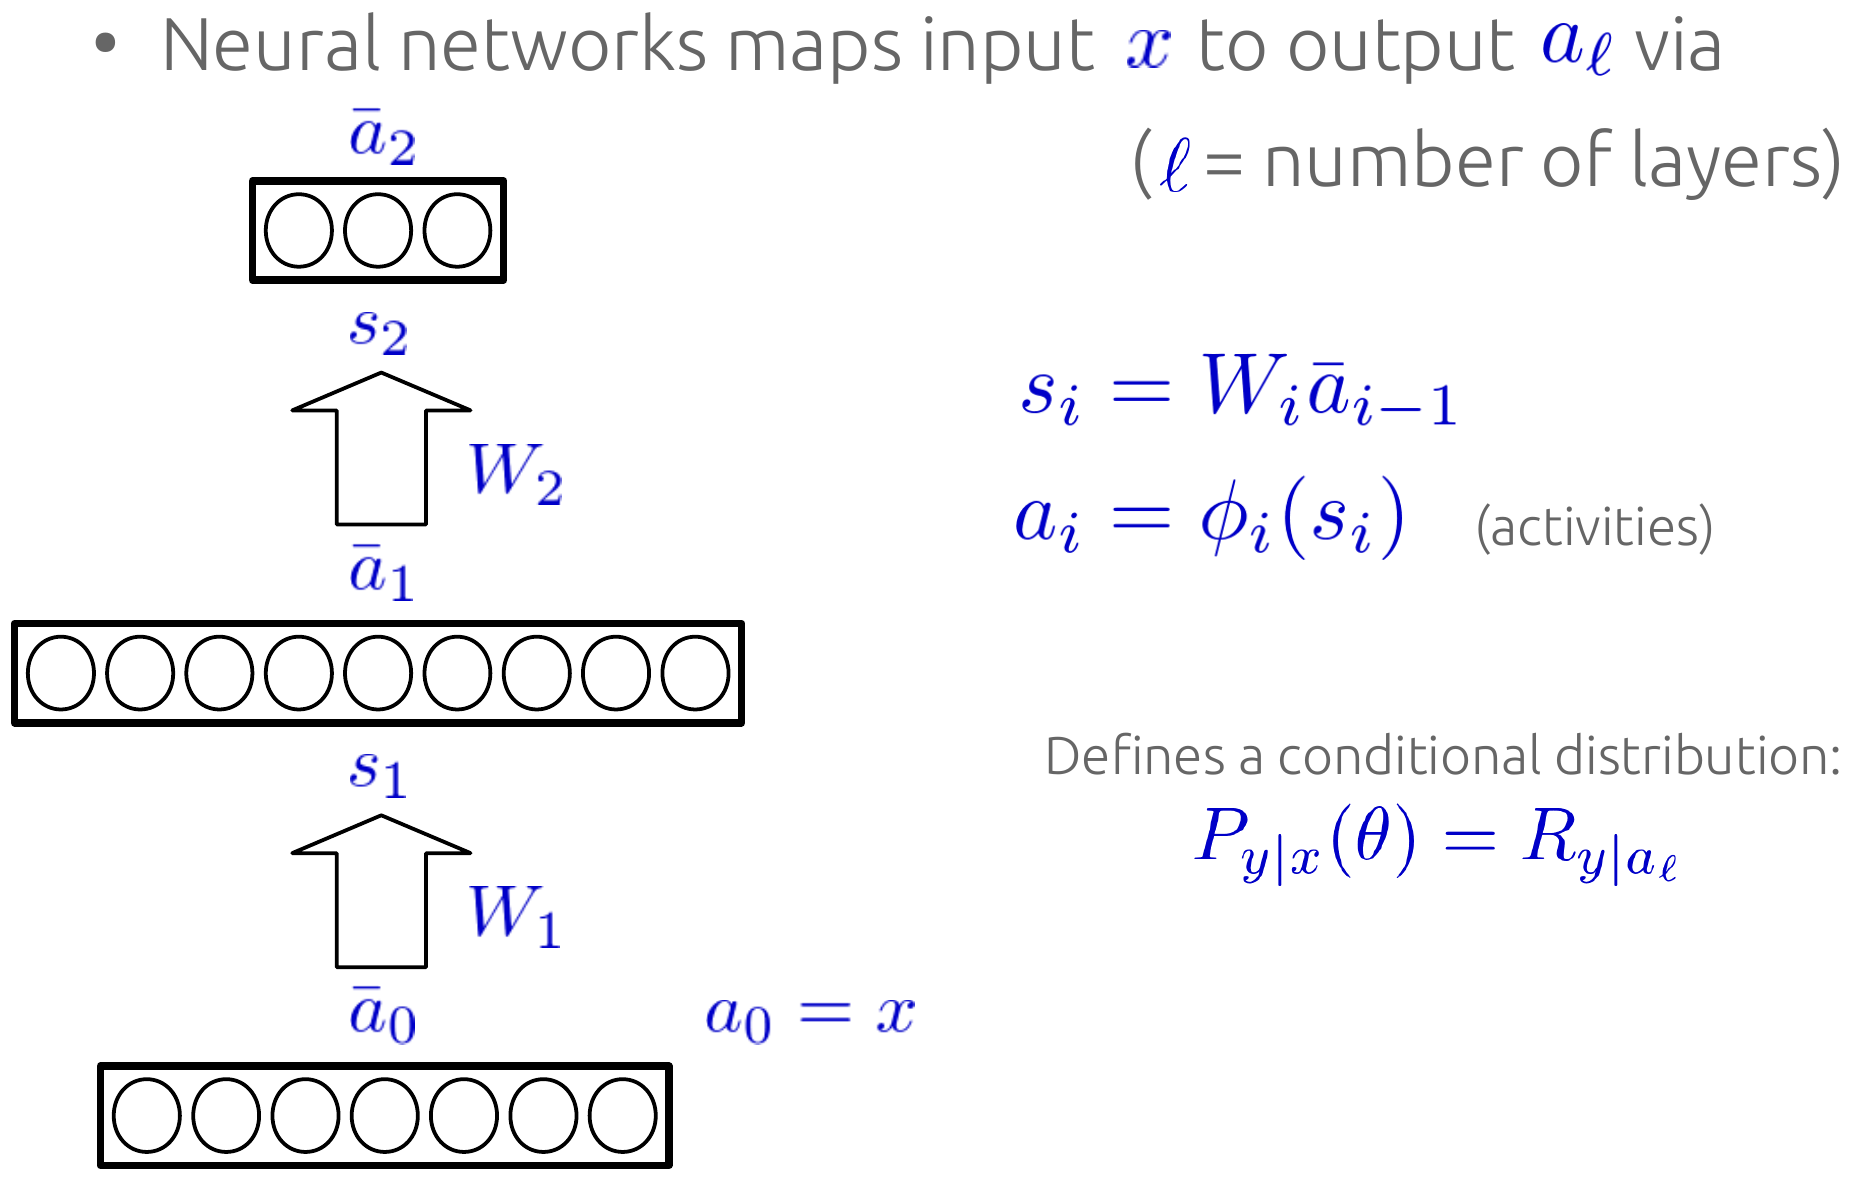
\includegraphics[scale=0.2]{net}
\end{figure}

$\bar{a}_i$: $a_i$ appended by a homogeneous coordinate with value 1,
to capture biar parameters explicitly
\end{frame}

\begin{frame}
\frametitle{Introduction}

\begin{figure}
    \centering
    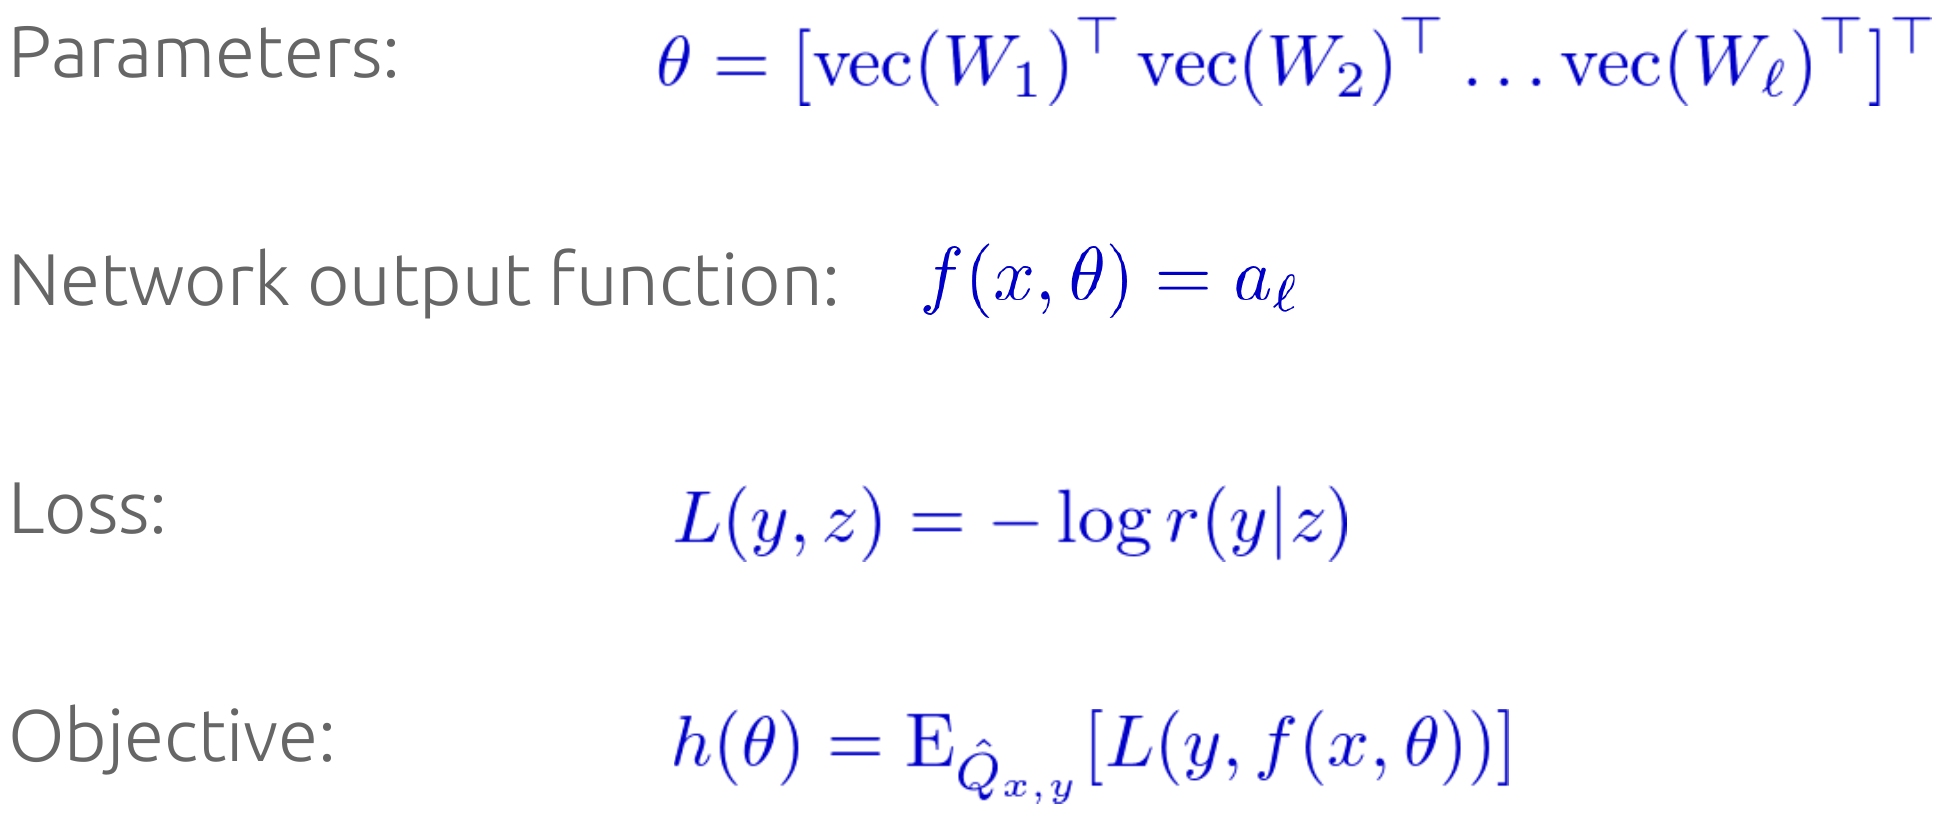
\includegraphics[scale=0.2]{net_param}
\end{figure}

\begin{itemize}
    \item $vec$ vectorizes matrices by stacking their columns together
    \item $\hat{Q}_{x, y}$: a training distribution
    \item $p(y|x, \theta) = r(y|f(x, \theta))$: the density function of $P_{y|x}(\theta) = R_{y|f(x,\theta)}$
\end{itemize}

\end{frame}

\begin{frame}
\frametitle{Introduction}
\begin{figure}
    \centering
    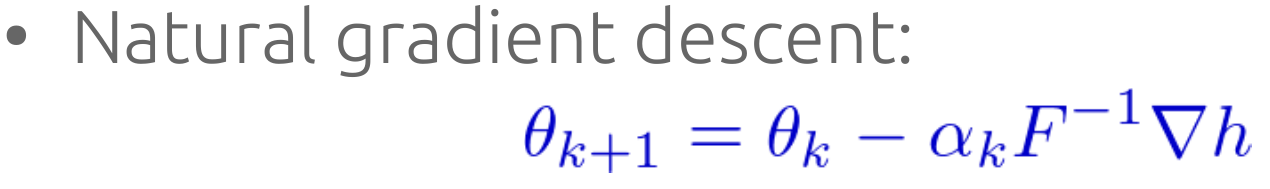
\includegraphics[scale=0.25]{natgrad}
\end{figure}

\begin{figure}
    \centering
    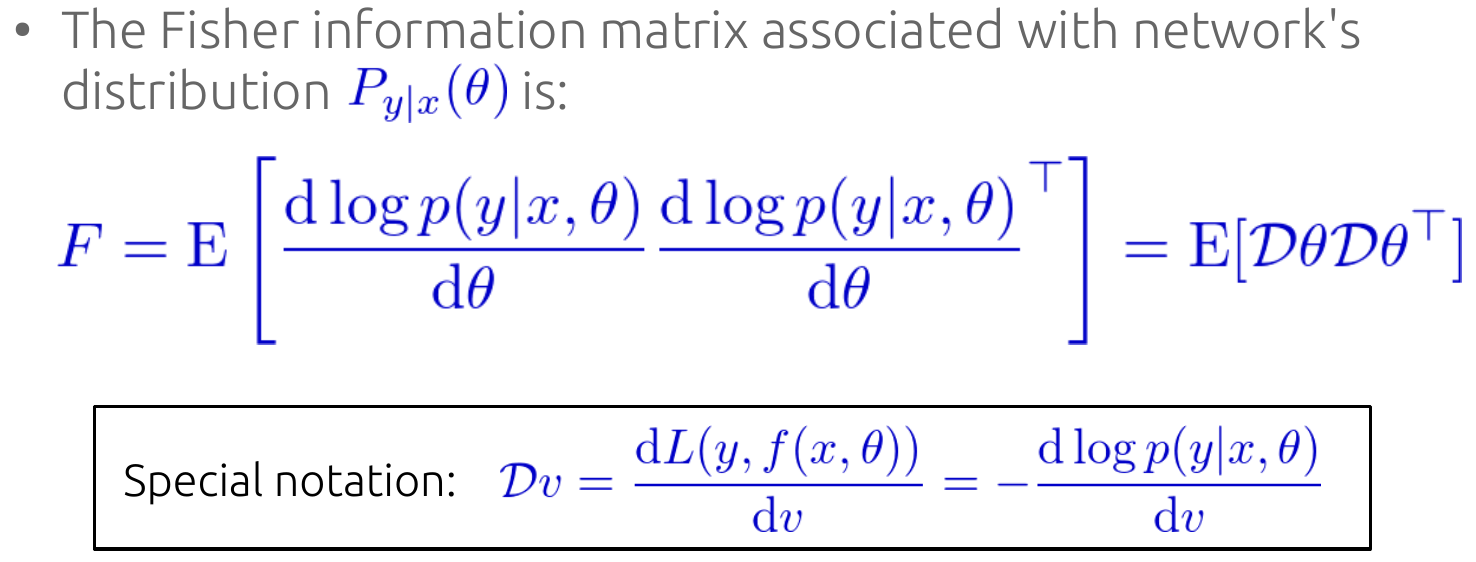
\includegraphics[scale=0.25]{fisher}
\end{figure}

\end{frame}
